\documentclass{article}
\usepackage{amsfonts}
\usepackage{amssymb}
\usepackage{pgfplots}
\pgfplotsset{compat=1.18}

\title{An Introduction to Complex Numbers}
\author{Joshua John Lee Shi Kai}

\begin{document}
\maketitle

\newpage

\section{Introduction}
Complex Analysis is quite similar to real analysis, except it works with complex numbers of the form
$x + iy$, where $x, y \in \mathbb{R}, i^2 = -1$. We represent real numbers on a line, we represent complex
numbers as elements on a plane.

\noindent \\ For example:
\begin{center}
	\begin{tikzpicture}
		\begin{axis}[xmin=0,xmax=3,ymin=0,ymax=3,xlabel = $x$, ylabel = $i$, axis lines = middle]
			\fill (2,1) circle[radius = 2pt] node[above right]{$(2,1)$};
		\end{axis}

	\end{tikzpicture}

\end{center}

\noindent A lot of complex analysis is really similar to real analysis, we can do the usual $+, -, \times, /$,
exponentials, trignometric functions, differentiation, integration. Many of the rules for real analysis work for
complex analysis. $\lim$, series and so on...

\subsection{Some Differences}
\subsubsection{Euler: $e^{ix} = cosx + isinx$}
Trigonometric functions and exponential functions turn out to be almost the same.
Using this we can write all trignometric functions in terms of exponential functions for example,
$cosx = \frac{e^{ix} + e^{-ix}}{2}$. This saves a lot of labour because all the complicated identities
for trigonometric functions are just special cases of identities of exponential functions. So there's a lot
less to remember.
\subsubsection{Differentiability}
For the reals, some functions we can differentiate it once and twice, but not three times. But for a
complex function $\mathbb{C} \rightarrow \mathbb{C}$, once it is differentiable once, it is automatically
differentiable any number of times.
\subsubsection{Integration}
Suppose we want to integrate
\begin{displaymath}
	\int_{0}^{1}f(x)dx
\end{displaymath}
Suppose we want to integrate for real numbers, and there's only one way to go from 0 to 1.
\begin{center}
	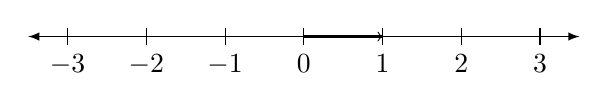
\begin{tikzpicture}
		\draw[latex-latex] (-3.5,0) -- (3.5,0) ; %edit here for the axis
		\foreach \x in  {-3,-2,-1,0,1,2,3} % edit here for the vertical lines
		\draw[shift={(\x,0)},color=black] (0pt,3pt) -- (0pt,-3pt);
		\foreach \x in {-3,-2,-1,0,1,2,3} % edit here for the numbers
		\draw[shift={(\x,0)},color=black] (0pt,0pt) -- (0pt,-3pt) node[below]
		{$\x$};
		\draw[->] (0,0) -- (1.0,0);
		\draw[very thick] (0,0) -- (1,0);
	\end{tikzpicture}
\end{center}
So its quite clear what this integral is meant.

\noindent \\ But if we are integrating in the complex plane,
\begin{center}
	\begin{tikzpicture}
		\begin{axis}[xmin=0,xmax=3,ymin=0,ymax=3,xlabel = $x$, ylabel = $i$, axis lines = middle]
			\fill (1,0) circle[radius = 2pt] node[above right]{$(1,0)$};
			\fill (0,1) circle[radius = 2pt] node[above right]{$(0,1)$};
		\end{axis}
	\end{tikzpicture}
\end{center}
There are many ways to go from 0 to 1. So the integral from 0 to 1 seems to depend on which path you take.
Turns out that it almost doesn't. We have Cauch's theorem, that integrals are almost independent of the path
we take from 0 to 1. This turns out to extremely useful. For example in real analysis

\begin{displaymath}
	\int_{0}^{\inf}
\end{displaymath}


\end{document}
